\documentclass{article}\usepackage[]{graphicx}\usepackage[]{color}
% maxwidth is the original width if it is less than linewidth
% otherwise use linewidth (to make sure the graphics do not exceed the margin)
\makeatletter
\def\maxwidth{ %
  \ifdim\Gin@nat@width>\linewidth
    \linewidth
  \else
    \Gin@nat@width
  \fi
}
\makeatother

\definecolor{fgcolor}{rgb}{0.345, 0.345, 0.345}
\newcommand{\hlnum}[1]{\textcolor[rgb]{0.686,0.059,0.569}{#1}}%
\newcommand{\hlstr}[1]{\textcolor[rgb]{0.192,0.494,0.8}{#1}}%
\newcommand{\hlcom}[1]{\textcolor[rgb]{0.678,0.584,0.686}{\textit{#1}}}%
\newcommand{\hlopt}[1]{\textcolor[rgb]{0,0,0}{#1}}%
\newcommand{\hlstd}[1]{\textcolor[rgb]{0.345,0.345,0.345}{#1}}%
\newcommand{\hlkwa}[1]{\textcolor[rgb]{0.161,0.373,0.58}{\textbf{#1}}}%
\newcommand{\hlkwb}[1]{\textcolor[rgb]{0.69,0.353,0.396}{#1}}%
\newcommand{\hlkwc}[1]{\textcolor[rgb]{0.333,0.667,0.333}{#1}}%
\newcommand{\hlkwd}[1]{\textcolor[rgb]{0.737,0.353,0.396}{\textbf{#1}}}%
\let\hlipl\hlkwb

\usepackage{framed}
\makeatletter
\newenvironment{kframe}{%
 \def\at@end@of@kframe{}%
 \ifinner\ifhmode%
  \def\at@end@of@kframe{\end{minipage}}%
  \begin{minipage}{\columnwidth}%
 \fi\fi%
 \def\FrameCommand##1{\hskip\@totalleftmargin \hskip-\fboxsep
 \colorbox{shadecolor}{##1}\hskip-\fboxsep
     % There is no \\@totalrightmargin, so:
     \hskip-\linewidth \hskip-\@totalleftmargin \hskip\columnwidth}%
 \MakeFramed {\advance\hsize-\width
   \@totalleftmargin\z@ \linewidth\hsize
   \@setminipage}}%
 {\par\unskip\endMakeFramed%
 \at@end@of@kframe}
\makeatother

\definecolor{shadecolor}{rgb}{.97, .97, .97}
\definecolor{messagecolor}{rgb}{0, 0, 0}
\definecolor{warningcolor}{rgb}{1, 0, 1}
\definecolor{errorcolor}{rgb}{1, 0, 0}
\newenvironment{knitrout}{}{} % an empty environment to be redefined in TeX

\usepackage{alltt}
\IfFileExists{upquote.sty}{\usepackage{upquote}}{}
\begin{document}




Load necessary libraries:
\begin{knitrout}
\definecolor{shadecolor}{rgb}{0.969, 0.969, 0.969}\color{fgcolor}\begin{kframe}
\begin{alltt}
\hlkwd{library}\hlstd{(RColorBrewer)}
\hlkwd{library}\hlstd{(plotrix)}
\end{alltt}


{\ttfamily\noindent\color{warningcolor}{\#\# Warning: package 'plotrix' was built under R version 4.0.3}}\begin{alltt}
\hlcom{##greys <- brewer.pal(8, "Greys")}
\hlstd{greys} \hlkwb{<-} \hlkwd{grey.colors}\hlstd{(}\hlnum{60}\hlstd{,} \hlkwc{start}\hlstd{=}\hlnum{1}\hlstd{,}\hlkwc{end}\hlstd{=}\hlnum{0}\hlstd{,} \hlkwc{gamma}\hlstd{=}\hlnum{1}\hlstd{)} \hlcom{##0=black, 1=white}

\hlstd{reds.func} \hlkwb{<-} \hlkwd{colorRampPalette}\hlstd{(}\hlkwd{c}\hlstd{(}\hlstr{"#FFFFFF"}\hlstd{,}\hlstr{"#FF0000"}\hlstd{))}
\hlstd{reds} \hlkwb{<-} \hlkwd{reds.func}\hlstd{(}\hlnum{60}\hlstd{)}
\end{alltt}
\end{kframe}
\end{knitrout}

Consider $2\times 2$ region representing the allowable space for $p_{11} \times p_{21}$:
\begin{knitrout}
\definecolor{shadecolor}{rgb}{0.969, 0.969, 0.969}\color{fgcolor}\begin{kframe}
\begin{alltt}
\hlcom{##gamma1argMax in terms of p11 and p21}
\hlstd{gamma1argMax} \hlkwb{<-} \hlkwa{function}\hlstd{(}\hlkwc{p11}\hlstd{,} \hlkwc{p21}\hlstd{)}
\hlstd{\{}
  \hlkwa{if}\hlstd{(((p21} \hlopt{>} \hlstd{p11)} \hlopt{&} \hlstd{(}\hlkwd{max}\hlstd{(p11, p21)} \hlopt{<=} \hlnum{1}\hlopt{/}\hlnum{2}\hlstd{))} \hlopt{|}
     \hlstd{((p11} \hlopt{>} \hlstd{p21)} \hlopt{&} \hlstd{(}\hlkwd{min}\hlstd{(p11, p21)} \hlopt{>=} \hlnum{1}\hlopt{/}\hlnum{2}\hlstd{)))}
  \hlstd{\{}
    \hlstd{gamma1argMax} \hlkwb{<-} \hlnum{0}
  \hlstd{\}} \hlkwa{else} \hlstd{\{}
    \hlkwa{if}\hlstd{(((p11} \hlopt{>} \hlstd{p21)} \hlopt{&} \hlstd{(}\hlkwd{max}\hlstd{(p11, p21)} \hlopt{<=} \hlnum{1}\hlopt{/}\hlnum{2}\hlstd{))} \hlopt{|}
       \hlstd{((p21} \hlopt{>} \hlstd{p21)} \hlopt{&} \hlstd{(}\hlkwd{min}\hlstd{(p11, p21)} \hlopt{>=} \hlnum{1}\hlopt{/}\hlnum{2}\hlstd{)))}
    \hlstd{\{}
      \hlstd{gamma1argMax} \hlkwb{<-} \hlnum{1}
    \hlstd{\}}
    \hlkwa{else} \hlstd{\{}
      \hlstd{gamma1argMax} \hlkwb{<-} \hlstd{(}\hlnum{1}\hlopt{-}\hlnum{2}\hlopt{*}\hlstd{p21)}\hlopt{/}\hlstd{(}\hlnum{2}\hlopt{*}\hlstd{(p11}\hlopt{-}\hlstd{p21))}
    \hlstd{\}}
  \hlstd{\}}
  \hlstd{gamma1argMax}
\hlstd{\}}

\hlcom{##p21 in terms of p11 and gamma1Star}
\hlstd{p21} \hlkwb{<-} \hlkwa{function}\hlstd{(}\hlkwc{p11}\hlstd{,} \hlkwc{gamma1Star}\hlstd{)}
\hlstd{\{}
  \hlstd{(}\hlnum{2}\hlopt{*}\hlstd{gamma1Star}\hlopt{*}\hlstd{p11}\hlopt{-}\hlnum{1}\hlstd{)}\hlopt{/}\hlstd{(}\hlnum{2}\hlopt{*}\hlstd{(gamma1Star}\hlopt{-}\hlnum{1}\hlstd{))}
\hlstd{\}}
\end{alltt}
\end{kframe}
\end{knitrout}

Make plot:
\begin{knitrout}
\definecolor{shadecolor}{rgb}{0.969, 0.969, 0.969}\color{fgcolor}\begin{kframe}
\begin{alltt}
\hlkwd{par}\hlstd{(}\hlkwc{mar}\hlstd{=}\hlkwd{c}\hlstd{(}\hlnum{7}\hlstd{,}\hlnum{4}\hlstd{,}\hlnum{4}\hlstd{,}\hlnum{6}\hlstd{))}
\hlkwd{plot}\hlstd{(}\hlnum{1}\hlstd{,} \hlkwc{type}\hlstd{=}\hlstr{"n"}\hlstd{,}
     \hlkwc{xlab}\hlstd{=}\hlkwd{expression}\hlstd{(p[}\hlnum{11}\hlstd{]),}
     \hlkwc{ylab}\hlstd{=}\hlkwd{expression}\hlstd{(p[}\hlnum{21}\hlstd{]),}
     \hlkwc{xlim}\hlstd{=}\hlkwd{c}\hlstd{(}\hlnum{0}\hlstd{,} \hlnum{1}\hlstd{),} \hlkwc{ylim}\hlstd{=}\hlkwd{c}\hlstd{(}\hlnum{0}\hlstd{,} \hlnum{1}\hlstd{),}
     \hlkwc{cex.axis}\hlstd{=}\hlnum{1.3}\hlstd{,}
     \hlkwc{cex.lab}\hlstd{=}\hlnum{1.3}\hlstd{,}
     \hlkwc{xaxt}\hlstd{=}\hlstr{"n"}\hlstd{,}
     \hlkwc{yaxt}\hlstd{=}\hlstr{"n"}\hlstd{)}

\hlkwd{axis}\hlstd{(}\hlnum{1}\hlstd{,} \hlkwc{at}\hlstd{=}\hlkwd{c}\hlstd{(}\hlnum{0}\hlstd{,}\hlnum{0.25}\hlstd{,}\hlnum{0.5}\hlstd{,}\hlnum{0.75}\hlstd{,}\hlnum{1}\hlstd{),}
     \hlkwc{cex.axis}\hlstd{=}\hlnum{1.3}\hlstd{)}
\hlkwd{axis}\hlstd{(}\hlnum{2}\hlstd{,} \hlkwc{at}\hlstd{=}\hlkwd{c}\hlstd{(}\hlnum{0}\hlstd{,}\hlnum{0.25}\hlstd{,}\hlnum{0.5}\hlstd{,}\hlnum{0.75}\hlstd{,}\hlnum{1}\hlstd{),}
     \hlkwc{cex.axis}\hlstd{=}\hlnum{1.3}\hlstd{)}

\hlcom{#color in grey the part that corresponds to max = 1}
\hlkwd{polygon}\hlstd{(}\hlkwd{c}\hlstd{(}  \hlnum{0}\hlstd{,}\hlnum{0.5}\hlstd{,}\hlnum{0.5}\hlstd{),}
        \hlkwd{c}\hlstd{(}  \hlnum{0}\hlstd{,}  \hlnum{0}\hlstd{,}\hlnum{0.5}\hlstd{),}
        \hlkwc{col}\hlstd{=greys[}\hlnum{10}\hlstd{],}
        \hlkwc{border}\hlstd{=}\hlnum{NA}\hlstd{)}
\hlkwd{polygon}\hlstd{(}\hlkwd{c}\hlstd{(}\hlnum{0.5}\hlstd{,}\hlnum{0.5}\hlstd{,}  \hlnum{1}\hlstd{),}
        \hlkwd{c}\hlstd{(}\hlnum{0.5}\hlstd{,}  \hlnum{1}\hlstd{,}  \hlnum{1}\hlstd{),}
        \hlkwc{col}\hlstd{=greys[}\hlnum{10}\hlstd{],}
        \hlkwc{border}\hlstd{=}\hlnum{NA}\hlstd{)}

\hlcom{##n = number of shades, excluding white and black (must be even number)}
\hlstd{n} \hlkwb{<-} \hlkwd{length}\hlstd{(reds)}\hlopt{-}\hlnum{2}

\hlkwa{for}\hlstd{(i} \hlkwa{in} \hlnum{1}\hlopt{:}\hlstd{(n}\hlopt{/}\hlnum{2}\hlstd{))}
\hlstd{\{}
  \hlkwd{polygon}\hlstd{(}\hlkwd{c}\hlstd{(}          \hlnum{0}\hlstd{,}      \hlnum{0}\hlstd{,}\hlnum{1}\hlopt{/}\hlnum{2}\hlstd{),}
          \hlkwd{c}\hlstd{(}\hlnum{1}\hlopt{/}\hlnum{2}\hlopt{+}\hlstd{(i}\hlopt{-}\hlnum{1}\hlstd{)}\hlopt{/}\hlstd{n,}\hlnum{1}\hlopt{/}\hlnum{2}\hlopt{+}\hlstd{i}\hlopt{/}\hlstd{n,}\hlnum{1}\hlopt{/}\hlnum{2}\hlstd{),}
          \hlkwc{col}\hlstd{=reds[i}\hlopt{+}\hlnum{1}\hlstd{],}
          \hlkwc{border} \hlstd{= reds[i}\hlopt{+}\hlnum{1}\hlstd{])}
  \hlkwd{polygon}\hlstd{(}\hlkwd{c}\hlstd{(}          \hlnum{1}\hlstd{,}      \hlnum{1}\hlstd{,}\hlnum{1}\hlopt{/}\hlnum{2}\hlstd{),}
          \hlkwd{c}\hlstd{(}\hlnum{1}\hlopt{/}\hlnum{2}\hlopt{-}\hlstd{(i}\hlopt{-}\hlnum{1}\hlstd{)}\hlopt{/}\hlstd{n,}\hlnum{1}\hlopt{/}\hlnum{2}\hlopt{-}\hlstd{i}\hlopt{/}\hlstd{n,}\hlnum{1}\hlopt{/}\hlnum{2}\hlstd{),}
          \hlkwc{col}\hlstd{=reds[i}\hlopt{+}\hlnum{1}\hlstd{],}
          \hlkwc{border}\hlstd{=reds[i}\hlopt{+}\hlnum{1}\hlstd{])}
\hlstd{\}}

\hlkwa{for}\hlstd{(i} \hlkwa{in} \hlnum{1}\hlopt{:}\hlstd{(n}\hlopt{/}\hlnum{2}\hlstd{))}
\hlstd{\{}
  \hlkwd{polygon}\hlstd{(}\hlkwd{c}\hlstd{((i}\hlopt{-}\hlnum{1}\hlstd{)}\hlopt{/}\hlstd{n,i}\hlopt{/}\hlstd{n,}\hlnum{1}\hlopt{/}\hlnum{2}\hlstd{),}
          \hlkwd{c}\hlstd{(}      \hlnum{1}\hlstd{,}  \hlnum{1}\hlstd{,}\hlnum{1}\hlopt{/}\hlnum{2}\hlstd{),}
          \hlkwc{col}\hlstd{=reds[i}\hlopt{+}\hlstd{(n}\hlopt{/}\hlnum{2}\hlstd{)}\hlopt{+}\hlnum{1}\hlstd{],}
          \hlkwc{border}\hlstd{=reds[i}\hlopt{+}\hlstd{(n}\hlopt{/}\hlnum{2}\hlstd{)}\hlopt{+}\hlnum{1}\hlstd{])}

  \hlkwd{polygon}\hlstd{(}\hlkwd{c}\hlstd{((n}\hlopt{-}\hlstd{i)}\hlopt{/}\hlstd{n,(n}\hlopt{+}\hlnum{1}\hlopt{-}\hlstd{i)}\hlopt{/}\hlstd{n,}\hlnum{1}\hlopt{/}\hlnum{2}\hlstd{),}
          \hlkwd{c}\hlstd{(}      \hlnum{0}\hlstd{,}  \hlnum{0}\hlstd{,}\hlnum{1}\hlopt{/}\hlnum{2}\hlstd{),}
          \hlkwc{col}\hlstd{=reds[i}\hlopt{+}\hlstd{(n}\hlopt{/}\hlnum{2}\hlstd{)}\hlopt{+}\hlnum{1}\hlstd{],}
          \hlkwc{border}\hlstd{=reds[i}\hlopt{+}\hlstd{(n}\hlopt{/}\hlnum{2}\hlstd{)}\hlopt{+}\hlnum{1}\hlstd{])}
\hlstd{\}}

\hlcom{##add some lines}
\hlstd{color_lines} \hlkwb{<-} \hlstr{"black"}
\hlkwd{abline}\hlstd{(}\hlkwc{h}\hlstd{=}\hlnum{0.5}\hlstd{,} \hlkwc{col}\hlstd{=color_lines,} \hlkwc{lwd}\hlstd{=}\hlnum{2}\hlstd{)}
\hlkwd{abline}\hlstd{(}\hlkwc{v}\hlstd{=}\hlnum{0.5}\hlstd{,} \hlkwc{col}\hlstd{=color_lines,} \hlkwc{lwd}\hlstd{=}\hlnum{2}\hlstd{)}
\hlkwd{abline}\hlstd{(}\hlkwc{a} \hlstd{=} \hlnum{0}\hlstd{,} \hlkwc{b}\hlstd{=}\hlnum{1}\hlstd{,} \hlkwc{col}\hlstd{=color_lines,} \hlkwc{lwd}\hlstd{=}\hlnum{2}\hlstd{)}

\hlkwd{text}\hlstd{(}\hlkwd{c}\hlstd{(}\hlnum{0.37}\hlstd{,} \hlnum{0.63}\hlstd{,} \hlnum{0.8}\hlstd{,} \hlnum{0.2}\hlstd{,} \hlnum{0.25}\hlstd{,} \hlnum{0.75}\hlstd{),}
     \hlkwd{c}\hlstd{(}\hlnum{0.2}\hlstd{,} \hlnum{0.8}\hlstd{,} \hlnum{0.63}\hlstd{,} \hlnum{0.37}\hlstd{,} \hlnum{0.8}\hlstd{,} \hlnum{0.2}\hlstd{),}
     \hlkwd{c}\hlstd{(}\hlstr{"max at 1"}\hlstd{,} \hlstr{"max at 1"}\hlstd{,}
       \hlstr{"max at 0"}\hlstd{,} \hlstr{"max at 0"}\hlstd{,}
       \hlkwd{expression}\hlstd{(}\hlkwd{paste}\hlstd{(}\hlstr{"max at "}\hlstd{,} \hlkwd{frac}\hlstd{(}\hlnum{1}\hlopt{-}\hlnum{2}\hlopt{*}\hlstd{p[}\hlnum{21}\hlstd{],}\hlnum{2}\hlopt{*}\hlstd{(p[}\hlnum{11}\hlstd{]}\hlopt{-}\hlstd{p[}\hlnum{21}\hlstd{])))),}
       \hlkwd{expression}\hlstd{(}\hlkwd{paste}\hlstd{(}\hlstr{"max at "}\hlstd{,} \hlkwd{frac}\hlstd{(}\hlnum{1}\hlopt{-}\hlnum{2}\hlopt{*}\hlstd{p[}\hlnum{21}\hlstd{],}\hlnum{2}\hlopt{*}\hlstd{(p[}\hlnum{11}\hlstd{]}\hlopt{-}\hlstd{p[}\hlnum{21}\hlstd{]))))),}
     \hlcom{##col=c("black","black","black","black","white","white"),}
     \hlkwc{cex}\hlstd{=}\hlnum{1.2}\hlstd{)}

\hlkwd{color.legend}\hlstd{(}\hlnum{1.1}\hlstd{,}\hlnum{0.35}\hlstd{,}\hlnum{1.2}\hlstd{,}\hlnum{0.65}\hlstd{,}
             \hlkwd{c}\hlstd{(}\hlnum{0}\hlstd{,}\hlnum{0.5}\hlstd{,}\hlnum{1}\hlstd{),}
             \hlstd{reds,}
             \hlkwc{align}\hlstd{=}\hlstr{"rb"}\hlstd{,}\hlkwc{gradient}\hlstd{=}\hlstr{"y"}\hlstd{,}
             \hlkwc{cex}\hlstd{=}\hlnum{1.3}\hlstd{)}
\end{alltt}
\end{kframe}
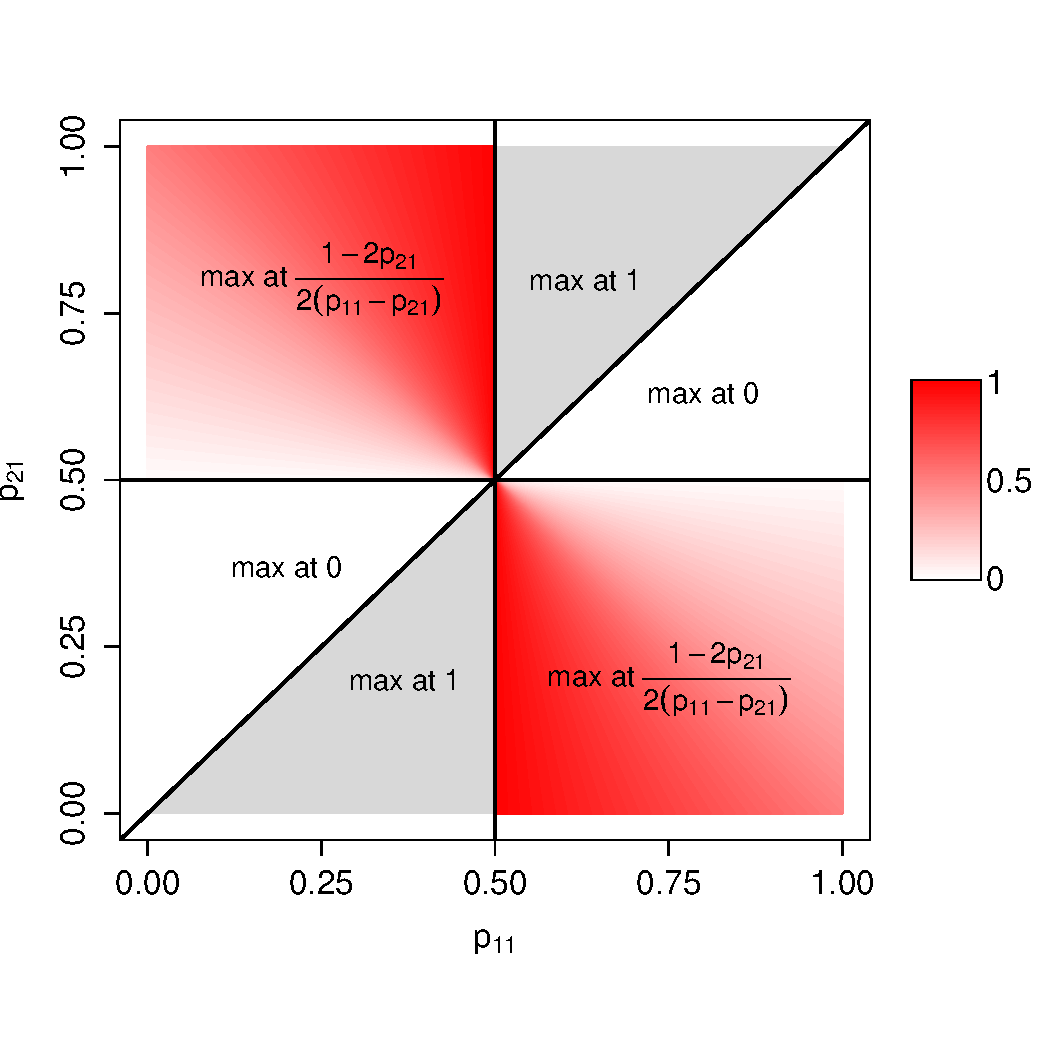
\includegraphics[width=\maxwidth]{../figs/Fig2-1} 

\end{knitrout}


\end{document}
